%\setcounter{chapter}{15}
\chapter{Категориальные типы}

В этой главе мы узнаем как в теории категорий 
определяются типы. В теории категорий типы
определяются как начальные и конечные объекты
в специальных категориях, которые называются алгебрами
функторов. Для понимания этой главы хорошо освежить в памяти
главу о структурной рекурсии, там где мы говорили
о свёртках и развёртках. 

\section{Программирование в стиле оригами}

Оригами -- состоит из двух слов \Quote{свёртка} и \Quote{бумага}. 
При программировании в стиле оригами все функции строятся
через функции свёртки и развёртки. Есть даже такие языки программрования,
в которых это единственный способ определения рекурсии.
Этот стиль очень хорошо подходит для ленивых языков программирования,
поскольку в связке:

\begin{code}
fold f . unfold g
\end{code}

\noindent функции свёртки и развёртки работают синхронно.
Функция развёртки не производит новых элементов до тех пор 
пока они не понадобятся во внешней функции свёртки.

Помните в одной из глав мы говорили о том, что рекурсивные
функции можно определять через функцию \In{fix}.  
Например так выглядит рекурсивная функция сложения всех чисел от 
одного до \In{n}:

\begin{code}
sumInt :: Int -> Int
sumInt 0 = 0
sumInt n = n + sumInt (n-1)
\end{code}

Эту функцию мы можем переписать с помощью функции \In{fix}.
При вычислении \In{fix f} будет составлено значение 

\begin{code}
f (f (f (f ...)))
\end{code}

Теперь перепишем функцию \In{sumInt} через \In{fix}:

\begin{code}
sumInt = fix $ \f n ->
    case n of 
        0   -> 0
        n   -> n + f (n - 1)    
\end{code}

Смотрите лямбда функция в аргументе \In{fix} 
принимает функцию и число, а возвращает число.
Тип этой функции \In{(Int -> Int) -> (Int -> Int)}.
После применения функции \In{fix} мы как раз и получим
функцию типа \In{Int -> Int}. В лямбда функции рекурсивный
вызов был заменён на вызов функции-параметра \In{f}. 

Оказывается, что этот приём может быть применён и 
для рекурсивных типов данных. Мы можем создать 
обобщённый тип, который обозначает рекурсивный тип:

\begin{code}
newtype Fix f = Fix { unFix :: f (Fix f) }
\end{code}

В этой записи мы получаем уравнение неподвижной точки 
\In{Fix f = f (Fix f)}, где \In{f} это некоторый тип с 
параметром. Определим тип целых чисел:

\begin{code}
data N a = Zero | Succ a

type Nat = Fix N
\end{code}

Теперь создадим несколько конструкторов:

\begin{code}
zero :: Nat
zero = Fix Zero

succ :: Nat -> Nat
succ = Fix . Succ
\end{code}

Сохраним эти определения в модуле \In{Fix.hs} и 
посмотрим в интерпретаторе на значения и их типы,
ghc не сможет вывести экземпляр \In{Show} для типа
\In{Fix}, потому что он зависит от типа с параметром,
а не от конкретного типа. Для решения этой проблемы
нам придётся определить экземпляры вручную и
подключить несколько расширений языка.
Помните в главе о ленивых вычислениях мы 
подключали расширение \In{BangPatterns}? 
Нам понадобятся:

\begin{code}
{-# Language FlexibleContexts, UndecidableInstances #-}
\end{code}

Теперь определим экземпляры для \In{Show} и \In{Eq}:

\begin{code}
instance Show (f (Fix f)) => Show (Fix f) where
    show x = "(" ++ show (unFix x) ++ ")"

instance Eq (f (Fix f)) => Eq (Fix f) where
    a == b = unFix a == unFix b
\end{code}

Определим списки-оригами:

\begin{code}
data L a b = Nil | Cons a b
    deriving (Show)

type List a = Fix (L a)

nil :: List a
nil = Fix Nil

infixr 5 `cons`

cons :: a -> List a -> List a
cons a = Fix . Cons a
\end{code}

В типе \In{L} мы заменили рекурсивный тип на параметр. 
Затем в записи \In{List a = Fix (L a)} мы производим замыкание 
по параметру. Мы бесконечно вкладываем тип \In{L a} во второй
параметр. Так получается рекурсивный тип для списков. 
Составим какой-нибудь список:

\begin{code}
*Fix> :r
[1 of 1] Compiling Fix              ( Fix.hs, interpreted )
Ok, modules loaded: Fix.
*Fix> 1 `cons` 2 `cons` 3 `cons` nil
(Cons 1 (Cons 2 (Cons 3 (Nil))))
\end{code}

Спрашивается, зачем нам это нужно? Зачем нам записывать
рекурсивные типы через тип \In{Fix}? Оказывается при такой
записи мы можем построить универсальные функции \In{fold} и \In{unfold},
они будут работать для любого рекурсивного типа.

Помните как мы составляли функции свёртки? Мы строили 
воображаемый класс, в котором сворачиваемый тип заменялся
на параметр. Например для списка мы строили свёртку так:

\begin{code}
class [a] b where
    (:) :: a -> b -> b
    []  :: b
\end{code}

После этого мы легко получали тип для функции свёртки:

\begin{code}
foldr :: (a -> b -> b) -> b -> ([a] -> b)
\end{code}

Она принимает методы воображаемого класса, в котором
тип записан с параметром, а возвращает функцию из
рекурсивного типа в тип параметра.

Сейчас мы выполняем эту процедуру замены рекурсивного 
типа на параметр в обратном порядке. Сначала мы строим типы с 
параметром, а затем получаем из них рекурсивные типы с помощью
конструкции \In{Fix}. Теперь методы класса с параметром это
наши конструкторы исходных классов, а рекурсивный тип записан
через \In{Fix}. Если мы сопоставим два способа, то мы сможем
получить такой тип для функции свёртки:

\begin{code}
fold :: (f b -> b) -> (Fix f -> b)
\end{code}

Смотрите функция свёртки по-прежнему принимает методы
воображаемого класса с параметром, но теперь класс перестал
быть воображаемым, он стал типом с параметром. Результатом
функции свёртки будет функция из рекурсивного типа \In{Fix f}
в тип параметр.

Аналогично строится и функция \In{unfold}:

\begin{code}
unfold :: (b -> f b) -> (b -> Fix f)
\end{code}

В первой функции мы указываем один шаг разворачивания
рекурсивного типа, а функция развёртки рекурсивно 
распространяет этот один шаг на потенциально бесконечную 
последовательность применений этого одного шага.

Теперь давайте определим эти функции. Но для этого 
нам понадобится от типа \In{f} одно свойство. Он должен быть 
функтором, опираясь на это свойство, мы будем рекурсивно
обходить этот тип.

\begin{code}
fold :: Functor f => (f a -> a) -> (Fix f -> a)
fold f = f . fmap (fold f) . unFix
\end{code}

Проверим эту функцию по типам. Для этого 
нарисуем схему композиции:

\begin{diagram}
\texttt{Fix f} && \rTo^{\texttt{unFix}} && \texttt{f (Fix f)} 
    && \rTo^{\texttt{fmap (fold f)}} && \texttt{f a} 
    && \rTo^{\texttt{f}} && \texttt{a} \\ 
\end{diagram}

Сначала мы разворачиваем обёртку \In{Fix} и получаем
значение типа \In{f (Fix f)}, затем с помощью \In{fmap}
мы внутри типа \In{f} рекурсивно вызываем функцию свёртки
и в итоге получаем значение \In{f a}, на последнем шаге 
мы выполняем свёртку на текущем уровне вызовом функции \In{f}.

Аналогично определяется и функция \In{unfold}. 
Только теперь мы сначала развернём первый уровень,
затем рекурсивно вызовем развёртку внутри типа \In{f}
и только в самом конце завернём всё в тип \In{Fix}:

\begin{code}
unfold :: Functor f => (a -> f a) -> (a -> Fix f)
unfold f = Fix . fmap (unfold f) . f
\end{code}

Схема композиции:

\begin{diagram}
\texttt{Fix f} && \lTo^{\texttt{Fix}} && \texttt{f (Fix f)} 
    && \lTo^{\texttt{fmap (unfold f)}} && \texttt{f a} 
    && \lTo^{\texttt{f}} && \texttt{a} \\ 
\end{diagram}

Возможно вы уже догадались о том, что функция \In{fold}
дуальна по отношению к функции \In{unfold}, это особенно
наглядно отражается на схеме композиции. При переходе от
\In{fold} к \In{unfold} мы просто перевернули все стрелки
заменили разворачивание типа \In{Fix} на заворачивание 
в \In{Fix}.

Определим несколько функций для натуральных чисел 
и списков в стиле оригами. Для начала сделаем \In{L}
и \In{N} экземпляром класса \In{Functor}:

\begin{code}
instance Functor N where
    fmap f x = case x of
        Zero    -> Zero
        Succ a  -> Succ (f a)

instance Functor (L a) where
    fmap f x = case x of
        Nil         -> Nil
        Cons a b    -> Cons a (f b)
\end{code}

Это всё что нам нужно для того чтобы начать пользоваться 
функциями свёртки и развёртки! Определим экземпляр \In{Num} 
для натуральных чисел:

\begin{code}
instance Num Nat where
    (+) a = fold $ \x -> case x of
            Zero    -> a
            Succ x  -> succ x

    (*) a = fold $ \x -> case x of
            Zero    -> zero
            Succ x  -> a + x

    fromInteger = unfold $ \n -> case n of
            0   -> Zero
            n   -> Succ (n-1)

    abs = undefined
    signum = undefined
\end{code}

Сложение и умножение определены через свёртку, а
функция построения натурального числа из числа 
типа \In{Integer} определена через развёртку. 
Сравните с теми функциями, которые мы писали в главе
про структурную рекурсию. Теперь мы не передаём отдельно
две функции, на которые мы будем заменять конструкторы.
Эти функции закодированы в типе с параметром.
Для того чтобы этот код заработал нам придётся добавить
ещё одно расширение \In{TypeSynonymInstances} наши
рекурсивные типы являются синонимами, а не новыми типами.
В рамках стандарта Haskell мы можем определять экземпляры
только для новых типов, для того чтобы обойти это ограничение
мы добавим ещё одно расширение. 

\begin{code}
*Fix> succ $ 1+2
(Succ (Succ (Succ (Succ (Zero)))))
*Fix> ((2 * 3) + 1) :: Nat
(Succ (Succ (Succ (Succ (Succ (Succ (Succ (Zero))))))))
*Fix> 2+2 == 2*(2::Nat)
True
\end{code}

Определим функции на списках. Для начала определим
две вспомогательные функции, которые извлекают голову и хвост списка:

\begin{code}
headL :: List a -> a
headL x = case unFix x of
    Nil         -> error "empty list"
    Cons a _    -> a

tailL :: List a -> List a
tailL x = case unFix x of
    Nil         -> error "empty list"
    Cons a b    -> b
\end{code}

Теперь определим несколько новых функций:

\begin{code}
mapL :: (a -> b) -> List a -> List b
mapL f = fold $ \x -> case x of
    Nil         -> nil
    Cons a b    -> f a `cons` b

takeL :: Int -> List a -> List a
takeL = curry $ unfold $ \(n, xs) -> 
    if n == 0 then Nil
              else Cons (headL xs) (n-1, tailL xs)
\end{code}

Сравните эти функции с теми, что мы определяли в главе 
о структурной рекурсии. Проверим работают ли эти функции:

\begin{code}
*Fix> :r
[1 of 1] Compiling Fix              ( Fix.hs, interpreted )
Ok, modules loaded: Fix.
*Fix> takeL 3 $ iterateL (+1) zero
(Cons (Zero) (Cons (Succ (Zero)) (Cons (Succ (Succ (Zero))) (Nil))))
*Fix> let x = 1 `cons` 2 `cons` 3 `cons` nil
*Fix> mapL (+10) $ x `concatL` x
(Cons 11 (Cons 12 (Cons 13 (Cons 11 (Cons 12 (Cons 13 (Nil)))))))
\end{code}

Обратите внимание, на то что с большими буквами мы пишем
\In{Cons} и \In{Nil} когда хотим закодировать функции 
для свёртки-развёртки, а с маленькой буквы пишем значения
рекурсивного типа. Надеюсь, что вы разобрались на примерах
как устроены функции \In{fold} и \In{unfold}, потому что
теперь мы перейдём к теории, которая за этим стоит.

\section{Индуктивные и коиндуктивные типы}

С точки зрения теории категорий функция свёртки
является катаморфизмом, а функция развёртки -- анаморфизмом.
Напомню, что катаморфизм -- это функция которая ставит
в соответствие объектам категории с начальным объектом
стрелки, которые начинаются из начального объекта, а 
заканчиваются в данном объекте. Анаморфизм -- это
перевёрнутый наизнанку катаморфизм.

Начальным и конечным объектом будет рекурсивный тип.
Вспомним тип свёртки:

\begin{code}
fold :: Functor f => (f a -> a) -> (Fix f -> a)
\end{code}

Функция свёртки строит функции, которые ведут из рекурсивного
типа в произвольный тип, поэтому в данном случае рекурсивный тип будет
начальным объектом. Функция развёртки строит из произвольного типа
данный рекурсивный тип, на языке теории категорий
она строит стрелку из произвольного объекта в рекурсивный,
это означает что  рекурсивный тип будет конечным объектом.

\begin{code}
unfold :: Functor f => (a -> f a) -> (a -> Fix f)
\end{code}

Категории, которые определяют рекурсивные типы таким образом
называются (ко)алгебрами функторов. Видите в типе и той и другой
функции стоит требование о том, что \In{f} является функтором.
Катаморфизм и анаморфизм отображают объекты в стрелки.
По типу функций \In{fold} и \In{unfold} мы можем сделать вывод,
что объектами в нашей категории будут стрелки вида 

\begin{code}
f a -> a
\end{code}

или для свёрток:

\begin{code}
a -> f a
\end{code}

А стрелками будут обычные функции одного аргумента. 
Теперь дадим более формальное определение. 

Эндофунктор $F : \CatA \Ra \CatA$ определяет
стрелки  $\alpha : FA \Ra A$, которые называется $F$-\emph{алгебрами}. 
Стрелку $h : A \Ra B$ называют \mbox{$F$-\emph{гомоморфизмом}}, 
если следующая диаграмма коммутирует: 

\begin{diagram}
FA           &  \rTo^{\alpha}   & A \\
\dTo^{Fh}    &                  & \dTo_{h} \\
FB           &  \rTo_{\beta}    & B \\
\end{diagram}

Или можно сказать по другому, для $F$-алгебр $\alpha:FA \Ra A$ 
и $\beta : FB \Ra B$ выполняется:

\[ Fh \Co \beta = \alpha \Co h   \]

Это свойство совпадает со свойством естественного 
преобразования только вместо одного из функторов мы подставили 
тождественный функтор $I$. 
Определим категорию $\Alg$, для категории $\CatA$ и 
эндофунктора $F : \CatA \Ra \CatA$

\begin{itemize}
\item Объектами являются $F$-алгебры $FA \Ra A$, где $A$ -- объект
    категории $\CatA$

\item Два объекта $\alpha : FA \Ra A$ и $\beta : FB \Ra B$ 
    соединяет $F$-гомоморфизм
    \mbox{$h : A \Ra B$}. Это такая стрелка из $\CatA$, для 
    которой выполняется:

\[ Fh \Co \beta = \alpha \Co h   \]

\item Композиция и тождественная стрелка взяты из категории $\CatA$.
\end{itemize}

Если в этой категории есть начальный объект $in_F : FT \Ra T$,
то определён катаморфизм, который переводит объекты $FA \Ra A$
в стрелки $T \Ra A$. Причём следующая диаграмма коммутирует:

\begin{diagram}
FT           &  \rTo^{in_F}   & T \\
\dTo^{F\cata{\alpha}}    &                  & \dTo_{\cata{\alpha}} \\
FA           &  \rTo_{\alpha}    & A \\
\end{diagram}

Этот катаморфизм и будет функцией свёртки для рекурсивного
типа $Т$. Понятие $\Alg$  можно перевернуть и получить 
категорию $\CoAlg$.

\begin{itemize}
\item Объектами являются $F$-коалгебры $A \Ra FA$, где $A$ -- объект
    категории $\CatA$

\item Два объекта $\alpha : FA \Ra A$ и $\beta : FB \Ra B$ 
    соединяет $F$-когомоморфизм
    \mbox{$h : A \Ra B$}. Это такая стрелка из $\CatA$, для 
    которой выполняется:

\[  h \Co \alpha = \beta \Co Fh  \]

\item Композиция и тождественная стрелка взяты из категории $\CatA$.
\end{itemize}

Если в этой категории есть конечный объект, его называют 
$out_F : T \Ra FT$, то определён анаморфизм, который
переводит объекты $A \Ra FA$ в стрелки $A \Ra T$.  
Причём следующая диаграмма коммутирует:

\begin{diagram}
T           &  \rTo^{in_F}   & FT \\
\dTo^{\ana{\alpha}}    &                  & \dTo_{F\ana{\alpha}} \\
A           &  \rTo_{\alpha}    & FA \\
\end{diagram}

Если для категории $\CatA$ и функтора
$F$ определены стрелки $in_F$  и $out_F$, то они
являются взаимнообратными и определяют изоморфизм $T \cong FT$.
Часто объект $T$ в случае $\Alg$ обозначают $\mu_F$, поскольку 
начальный объект определяется функтором $F$, а в случае $\CoAlg$
обозначают $\nu_F$. 

Типы, которые являются начальными объектами, принято 
называть индуктивными, а типы, которые являются конечными
объектами -- коиндуктивными. 

\subsection{Существование начальных и конечных объектов}

Мы говорили, что если начальный(конечный) объект существует,
а когда он существует? Рассмотрим один важный случай. 
Если категория является категорией, в которой объектами 
являются полные частично упорядоченные множества, а стрелками
являются монотонные функции, такие категории называют
$\textbf{CPO}$, и функтор -- полиномиальный,
то начальный и конечный объекты существуют.

\subsubsection{Полные частично упорядоченные множества}

Оказывается на значениях можно ввести частичный порядок.
Порядок называется частичным, если отношение $\leq$ 
определено не для всех элементов, а  лишь для
некоторых из них. Частичный порядок на значениях
отражает степень неопределённости значения. 
Самый маленький объект это полностью неопределённое
значение $\bot$. Любое значение типа содержит больше 
определённости чем $\bot$.

Для того чтобы не путать упорядочивание 
значений по степени определённости с обычным числовым порядком,
пользуются специальным символом $\sqsubseteq$. Запись 

\[ a \sqsubseteq b \]

\noindent означает, что $b$ более определено (или информативнее) чем $a$.


Так для логических значений определены два нетривиальных 
сравнения: 

\[ data\ Bool\ =\ True \Or False \]

\[ \bot \sqsubseteq True \]
\[ \bot \sqsubseteq False \]



Мы будем называть нетривиальными сравнения в которых, компоненты
слева и справа от $\sqsubseteq$ не равны. Например ясно, что 
$True \sqsubseteq True$ или $\bot \leq \bot$. Это тривиальные 
сравнения и мы их будем лишь подразумевать. Считается, что
если два значения определены полностью, то мы не можем
сказать какое из них информативнее. Так к примеру для логических
значений мы не можем сказать какое значение более определено
$True$ или $False$.

Рассмотрим пример по-сложнее. Частично определённые значения:

\[ data\ Maybe\ a = Nothing \Or Just\ a \]


\[\begin{array}{l@{\ \sqsubseteq \ }l}
    \bot & Nothing \\
    \bot & Just\ \bot \\
    \bot & Just\ a \\
    Just\ a & Just\ b,\qquad \text{если } a \sqsubseteq b    
\end{array}\]

Если вспомнить как происходит вычисление значения, 
то значение $a$ менее определено чем $b$, если взрывное
значение $\bot$ в $a$ находится ближе к корню значения, 
чем в $b$. Итак получается, что в категории $\textbf{Hask}$
объекты это множества с частичным порядком. 
Что означает требование монотонности функции?  
Монотонность в контексте операции $\sqsubseteq$
говорит о том, что чем больше определён вход функции
тем больше определён выход:

\[ a \sqsubseteq b \quad \RA \quad f\ a \sqsubseteq f\ b \]

Это требование накладывает запрет на возможность проведения
сопоставления с образцом по значению $\bot$. Иначе мы можем
определять немонотонные функции вроде:


\begin{code}
isBot :: Bool -> Bool
isBot undefined = True
isBot _         = undefined
\end{code}

Полнота частично упорядоченного множества означает,
что у любой последовательности $x_n$ 

\[ x_0 \sqsubseteq x_1 \sqsubseteq x_2 \sqsubseteq \dots \]

\noindent есть значение $x$, к которому она сходится.
Это значение называют супремумом множества.
Что такое полные частично упорядоченные множества 
мы разобрались. А что такое полиномиальный функтор? 

\subsubsection{Полиномиальный функтор}

Полиномиальный функтор -- это функтор который построен лишь
с помощью операций суммы, произведения, постоянных функторов,
тождественного фуктора и композиции функторов.
Определим эти операции:

\begin{itemize}
\item Сумма функторов $F$ и $G$ определяется через операцию
    суммы объектов:

   \[ (F+G)X = FX + GX \]
        
\item Произведение функторов $F$ и $G$ определяется через операцию 
    произведения объектов:

    \[ (F\times G)X = FX \times GX \]

\item Постоянный функтор отображает все объекты категории 
    в один объект, а стрелки в тождественнубю стрелку этого
    объекта, мы будем обозначать постоянный функтор подчёркиванием:

\begin{eqnarray*}
    \underline{A}X &=& A \\
    \underline{A}f &=& id_A \\
\end{eqnarray*}

\item Тождественный функтор оставляет объекты и стрелки
    неизменными:

\begin{eqnarray*}
    IX &=& X \\
    If &=& f \\
\end{eqnarray*}
  
\item Композиция функторов $F$ и $G$ это последовательное применение 
     функторов

\[ FGX = F(GX) \]
\end{itemize}

По определению функции построенные с помощью этих операций
называют полиномиальными. 
Определим несколько типов данных с помощью полиномиальных
функторов. Определим логические значения:

\[ Bool = \mu(\underline{1} + \underline{1}) \]

Объект $1$ обозначает любую константу, это конечный объект
исходной категории. Нам не важны имена конструкторов,
но важна структура типа. $\mu$ обозначает начальный объект
в $F$-алгебре. 

Определим натуральные числа:

\[ Nat = \mu(\underline{1} + I) \]

Эта запись обозначает начальный объект для $F$-алгебры
с функтором $F=\underline{1}+I$. 
Посмотрим на определение списка:

\[ List_A = \mu(\underline{1} + \underline{A} \times I) \]

Список это начальный объект $F$-алгебры 
$\underline{1}+\underline{A}\times I$. 
Также можно определить бинарные деревья:

\[ BTree_A = \mu(\underline{A} + I \times I )\]

Определим потоки:

\[ Stream_A = \nu (\underline{A} \times I) \]

Потоки являются конечным объектом $F$-коалгебры, 
где $F= \underline{A} \times I$.

\section{Гиломорфизм}

Оказывается, что с помощью катаморфизма и анаморфизма
мы можем определить функцию \In{fix}, т.е.~мы можем
выразить любую рекурсивную функцию с помощью структурной
рекурсии. 

Функция \In{fix} строит бесконечную последовательность
применений некоторой функции \In{f}. 

\begin{code}
f (f (f ...)))
\end{code}

Сначала с помощью анаморфизма мы построим бесконечный список, 
который содержит функцию \In{f} во всех элементах:

\begin{code}
repeat f = f : f : f : ...
\end{code}

А затем заменим конструктор \In{:} на применение.
В итоге мы получим такую функцию:


\begin{code}
fix :: (a -> a) -> a
fix = foldr ($) undefined . repeat 
\end{code}

Убедимся, что эта функция работает:

\begin{code}
Prelude> let fix = foldr ($) undefined . repeat
Prelude> take 3 $ y (1:)
[1,1,1]
Prelude> fix (\f n -> if n==0 then 0 else n + f (n-1)) 10
55
\end{code}

Теперь давайте определим функцию \In{fix} через функции 
\In{cata} и \In{ana}:

\begin{code}
fix :: (a -> a) -> a
fix = cata (\(Cons f a) -> f a) . ana (\a -> Cons a a)
\end{code}


Эта связка анаморфизм с последующим катаморфизмом
встречается так часто, что ей дали специальное имя. 
\emph{Гиломорфизмом} называют функцию:

\begin{code}
hylo :: Functor f => (f b -> b) -> (a -> f a) -> (a -> b) 
hylo phi psi = cata phi . ana psi
\end{code}

Отметим, что эту функцию можно выразить и по-другому:

\begin{code}
hylo :: Functor f => (f b -> b) -> (a -> f a) -> (a -> b) 
hylo phi psi = phi . (fmap $ hylo phi psi) . psi
\end{code}

Этот вариант более эффективен по расходу памяти, мы не строим 
промежуточное значение \In{Fix f}, а сразу обрабатываем значения
в функции \In{phi} по ходу их построения в функции \In{psi}.
Давайте введём инфиксную операцию гиломорфизм для этого определения:

\begin{code}
(>>) :: Functor f => (a -> f a) -> (f b -> b) -> (a -> b) 
psi >> phi = phi . (fmap $ hylo phi psi) . psi
\end{code}

Теперь давайте скроем одноимённую
функцию из \In{Prelude} и определим несколько рекурсивных функций 
с помощью гиломорфизма.
Начнём с функции вычисления суммы чисел от нуля до данного числа:

\begin{code}
sumInt :: Int -> Int
sumInt = range >> sum
    
sum x = case x of
    Nil      -> 0 
    Cons a b -> a + b

range n 
    | n == 0    = Nil 
    | otherwise = Cons n (n-1)
\end{code}

Сначала мы создаём в функции \In{range} список 
всех чисел от данного числа до нуля. А затем в функции
\In{sum} складываем значения. Теперь мы можем легко
определить функцию вычисления факториала:

\begin{code}
fact :: Int -> Int
fact = range >> prod
    
prod x = case x of
    Nil      -> 1 
    Cons a b -> a * b
\end{code}

Напишем функцию, которая извлекает из потока n-тый элемент.
Сначала определим тип для потока:

\begin{code}
type Stream a = Fix (S a)

data S a b = a :& b
    deriving (Show, Eq)

instance Functor (S a) where
    fmap f (a :& b) = a :& f b  


headS :: Stream a -> a
headS x = case unFix x of
    (a :& _) -> a


tailS :: Stream a -> Stream a
tailS x = case unFix x of
    (_ :& b) -> b
\end{code}


Теперь функцию извлечения элемента:

\begin{code}
getElem :: Int -> Stream a -> a
getElem = curry (enum >> elem) 
    where elem ((n, a) :& next) 
                | n == 0    = a
                | otherwise = next
          enum (a, st) = (a, headS st) :& (a-1, tailS st)
\end{code}

В функции \In{enum} мы добавляем  к элементам потока
убывающую последовательность чисел, она стартует из данного
числа. Элемент, который нам нужен, будет содержать в этой последовательности
число ноль. В функции \In{elem} мы как раз и извлекаем тот элемент
рядом с которым хранится число ноль. Обратите внимание на то, что
рекурсия встроена в этот алгоритм, если данное число не равно нулю,
мы просто извлекаем следующий элемент.

С помощью этой функции мы можем вычислить n-тое число
из ряда чисел Фибоначчи. Сначала создадим поток чисел
Фибоначчи:

\begin{code}
fibs :: Stream Int
fibs = ana (\(a, b) -> a :& (b, a+b)) (0, 1)
\end{code}

Теперь просто извлечём n-тый элемент из потока
чисел Фибоначчи:

\begin{code}
fib :: Int -> Int
fib = flip getElem fibs
\end{code}

Вычислим поток всех простых чисел. Мы будем вычислять
его по алгоритму \Quote{решето Эратосфена}. В начале 
алгоритма у нас есть поток целых чисел и известно, что 
первое число является простым. 

\newcommand{\XEr}[1]{\text{\xout{#1}}}

\[ 2,\ 3,\ 4,\ 5,\ 6,\ 7,\ 8,\ 9,\ 10,\ 11,\ 12,\ 13,\ 14,\ 15\ \dots \]

В процессе этого алгоритма мы вычёркиваем все
не простые числа. Сначала мы ищем первое не зачёркнутое 
число и помещаем его в результирующий поток, а 
на следующий шаг алгоритма мы передаём исходный, поток в 
котором зачёркнуты все числа кратные тому, что мы положили 
последним:

\[ 2 \]
\[ \ 3,\ \XEr{4},\ 5,\ \XEr{6},\ 7,\ \XEr{8},\ 9,\ \XEr{10},\ 11,\ 
       \XEr{12},\ 13,\ \XEr{14},\ 15\  \dots \]

Теперь мы ищем первое незачёркнутое число и помещаем его
в результат. А на следующий шаг рекусии передаём поток,
в котором зачёркнуты все числа кратные новому простому числу:

\[ 2,\ 3 \]
\[ \ \XEr{4},\ 5,\ \XEr{6},\ 7,\ \XEr{8},\ \XEr{9},\ \XEr{10}\ 
       \XEr{12},\ 13,\ \XEr{14},\ \XEr{15}\  \dots \]

И так далее, на каждом шаге мы будем получать одно простое число.
Зачёркивание мы будем имитировать с помощью типа \In{Maybe}.
Всё начинается с потока целых чисел, в котором не зачёркнуто
ни одно число:

\begin{code}
nums :: Stream (Maybe Int)
nums = mapS Just $ iterateS (+1) 2 

mapS :: (a -> b) -> Stream a -> Stream b
mapS f = ana $ \xs -> (f $ headS xs) :& tailS xs

iterateS :: (a -> a) -> a -> Stream a
iterateS f = ana $ \x -> x :& f x
\end{code}

В силу ограничений системы типов Haskell мы не можем определить
экземпляр \In{Functor} для типа \In{Stream}, поскольку \In{Stream}
является не самостоятельным типом а типом-синонимом. Поэтому
нам приходится определить функцию \In{mapS}. Определим шаг
рекурсии:

\begin{code}
primes :: Stream Int
primes = ana erato nums

erato xs = n :& erase n ys
    where n  = fromJust $ headS xs  
          ys = dropWhileS isNothing xs
\end{code}

Переменная \In{n} содержит первое не зачёркнутое число
на данном шаге. Переменная \In{ys} указывает на список
чисел, из начала которого удалены все зачёркнутые числа.
Функции \In{isNothing} и \In{fromJust} взяты из 
стандартного модуля \In{Data.Maybe}.
Нам осталось определить лишь две функции. Это аналог
функции \In{dropWhile} на списках. Эта функция удаляет 
из начала списка все элементы, которые удовлетворяют некоторому
предикату. Вторая функция \In{erase} вычёркивает все 
числа в потоке кратные данному.

\begin{code}
dropWhileS :: (a -> Bool) -> Stream a -> Stream a
dropWhileS p = psi >> phi 
    where phi ((b, xs) :& next) = if b then next else xs
          psi xs = (p $ headS xs, xs) :& tailS xs
\end{code}

В этой функции мы сначала генерируем список пар, который
содержит значения предиката и остатки списка, а затем
находим в этом списке первый такой элемент, значение
которого равно \In{False}. 


\begin{code}
erase :: Int -> Stream (Maybe a) -> Stream (Maybe a)
erase n xs = ana phi (0, xs)
    where phi (a, xs) 
            | a == 0    = Nothing  :& (a', tailS xs)
            | otherwise = headS xs :& (a', tailS xs)
            where a' = if a == n-1 then 0 else (a+1)
\end{code}

В функции \In{erase} мы заменяем на \In{Nothing} каждый 
элемент, порядок следования которого кратен аргументу \In{n}.
Проверим, что у нас получилось:

\begin{code}
*Fix> primes 
(2 :& (3 :& (5 :& (7 :& (11 :& (13 :& (17 :& (19 :& (23 :& 
(29 :& (31 :& (37 :& (41 :& (43 :& (47 :& (53 :& (59 :& 
(61 :& (67 :& (71 :& (73 :& (79 :& (83 :& (89 :& (97 :& 
(101 :& (103 :& (107 :& (109 :& (113 :& (127 :& (131 :&
...
\end{code}

\section{Краткое содержание}

В этой главе мы узнали, что любая рекурсивная 
функция может быть выражена через структурную рекурсию.
Мы узнали как в теории категорий определяются типы. 
Типы являются начальными и конечными объектами в 
специальных категориях, которые называются алгебрами 
функторов. Слоган теории категорий гласит:

\begin{quote}
Управляющие структуры определяются структурой типов.
\end{quote}

Определив тип, мы получаем вместе с ним две функции
структурной рекурсии, это катаморфизм (для начальных объектов) 
и анаморфизм (для конечных объектов). С помощью катаморфизма
мы можем сворачивать значение данного типа в значения
любого другого типа, а с помощью анаморфизма
мы можем разворачивать значения данного типа из
значений любого другого типа. Также мы узнали, что 
категория $\textbf{Hask}$
является категорией $\textbf{CPO}$, категорией полных
частично упорядоченных множеств.

\section{Упражнения}

Потренируйтесь в определении рекурсивных функций через гиломорфизм.
Попробуйте переписать как можно больше определений из главы
о структурной рекурсии в терминах типа \In{Fix} и функций 
\In{cata}, \In{ana} и \In{hylo}. Также потренируйтесь
на стандартных функциях из модуля \In{Prelude}. Определите
новые типы через \In{Fix} например деревья из модуля
\In{Data.Tree}. Попробуйте свои силы на функциях по-сложнее
например алгоритме эвристического поиска.



\newcommand{\Dia}[1]{\fbox{\text{#1}}}

\begin{tikzpicture}[scale=5]
\draw (2,2) circle (1);
\end{tikzpicture}

\tikz \draw (0,0) --  +(1,0) --  +(0,1) --  +(1,1);

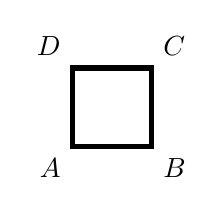
\begin{tikzpicture}[line width=2pt]
  \draw (0,0) node [below left]  {$A$} -- 
        (1,0) node [below right] {$B$} -- 
        (1,1) node [above right] {$C$} -- 
        (0,1) node [above left]  {$D$} -- 
        cycle;
\end{tikzpicture}

\begin{comment}
\begin{diagram}
 &          & \text{Файл .hs} \\
 &          & \dTo  \\
 &          & \Dia{Построение синтаксического дерева} \\
 &          & \dTo \\
 &          & \Dia{Разрешение имён} \\
 &          & \dTo \\
 &          & \Dia{Проверка типов} \\
 &          & \dTo \\
 &          & \Dia{Устранение синтаксического сахара} \\
 &          & \dTo^{\text{Core}} \\
 &          & \Dia{Упрощение Core}     & \rTo & \Dia{Генерация кода для ghci} \\
 &          & \dTo^{\text{STG}} \\
 &          & \Dia{Генерация Cmm} \\ 
 &          & \dTo \\
 &          & \Dia{Cmm}    &        &  \\
 & \ldTo    & \dTo          & \rdTo  &  \\
\Dia{C} &  & \Dia{Native} &        & \Dia{LLVM}  \\
\end{diagram}
\end{comment}


